%%
%% This is file `sample-sigconf.tex',
%% generated with the docstrip utility.
%%
%% The original source files were:
%%
%% samples.dtx  (with options: `sigconf')
%% 
%% IMPORTANT NOTICE:
%% 
%% For the copyright see the source file.
%% 
%% Any modified versions of this file must be renamed
%% with new filenames distinct from sample-sigconf.tex.
%% 
%% For distribution of the original source see the terms
%% for copying and modification in the file samples.dtx.
%% 
%% This generated file may be distributed as long as the
%% original source files, as listed above, are part of the
%% same distribution. (The sources need not necessarily be
%% in the same archive or directory.)
%%
%% The first command in your LaTeX source must be the \documentclass command.
\documentclass[sigconf,anonymous]{acmart}

\usepackage{libertine}
\usepackage{lipsum}% http://ctan.org/pkg/lipsum
\usepackage{algorithm}% http://ctan.org/pkg/algorithm
\usepackage{algpseudocode}% http://ctan.org/pkg/algorithmicx
\usepackage{graphicx}
\usepackage[compatibility=false]{caption}% http://ctan.org/pkg/caption
\usepackage{booktabs}
%% \usepackage{cite}
\usepackage{url}
\usepackage{multirow}
\usepackage{pgfplots}
\usepackage{tikz}
\usetikzlibrary{matrix,fit,shapes,calc,positioning,shadows,arrows,shapes,backgrounds,decorations.markings,fadings}
\usepackage{listings}
\usepackage[caption=false, font=footnotesize]{subfig}
\renewcommand{\ttdefault}{pcr}
\lstset{
  basicstyle=\scriptsize\ttfamily,
  keywordstyle=\scriptsize\ttfamily\bfseries,
  language=C,             % choose the language of the code
  frame=single,              % adds a frame around the code
  aboveskip=0pt,
  belowskip=0pt,
  breaklines=true,           % sets automatic line breaking
  breakatwhitespace=false,   % sets if automatic breaks should only happen at
  showspaces=false,
  %numbersep=5pt,              % Abstand der Nummern zum Text
  %tabsize=2,                  % Groesse von Tabs
  %extendedchars=true,         %
  %breaklines=true,            % Zeilen werden Umgebrochen
  keywords=[2]{tcp, flag, threshold, track, count, seconds, classtype, sid}
}
\usepackage{balance}
\usepackage{wrapfig}
\usepackage{enumitem}
\usepackage{color, colortbl}
\definecolor{Gray}{gray}{0.9}

%% 
\newcommand{\tname}{\textsc{Syrius}} %% name of the technique
\newcommand{\ie}{i.e.}
\newcommand{\eg}{e.g.}
\newcommand{\aka}{a.k.a.}
\newcommand{\etal}{and colleagues}
\newcommand{\nids}{NIDS}
\newcommand{\metas}{Metasploit}
\newcommand{\suri}{Suricata}
\newcommand{\numrulessuri}{27.8K}
\newcommand{\percRulesWithContent}{93.5\%}
\newcommand{\numundetected}{\Fix{XX\%}}
\newcommand{\CodeIn}[1]{{\small{\texttt{#1}}}}
\newcommand{\MyComment}[1]{}

%% review
\newcommand{\Fix}[1]{{\textbf{[[}\color{magenta}#1}\textbf{]]}}
\newcommand{\Mar}[1]{{\textbf{[[Marcelo:~}\color{red}#1}\textbf{]]}}
\newcommand{\Luc}[1]{{\textbf{[[Lucas:~}\color{blue}#1}\textbf{]]}}
\newcommand{\Gui}[1]{{\textbf{[[Guilherme:~}\color{green}#1}\textbf{]]}}

\def\denseitems{
   \itemsep1pt plus1pt minus1pt
   \parsep0pt plus0pt
   \parskip0pt\topsep0pt}

%% numbers
\newcommand{\totoptions}{162}
\newcommand{\numproto}{11}
\newcommand{\totoptionsrelevant}{153}


%%
%% \BibTeX command to typeset BibTeX logo in the docs
\AtBeginDocument{%
  \providecommand\BibTeX{{%
    \normalfont B\kern-0.5em{\scshape i\kern-0.25em b}\kern-0.8em\TeX}}}

%% Rights management information.  This information is sent to you
%% when you complete the rights form.  These commands have SAMPLE
%% values in them; it is your responsibility as an author to replace
%% the commands and values with those provided to you when you
%% complete the rights form.
\setcopyright{acmcopyright}
\copyrightyear{2018}
\acmYear{2018}
\acmDOI{10.1145/1122445.1122456}

%% These commands are for a PROCEEDINGS abstract or paper.
\acmConference[Woodstock '18]{Woodstock '18: ACM Symposium on Neural
  Gaze Detection}{June 03--05, 2018}{Woodstock, NY}
\acmBooktitle{Woodstock '18: ACM Symposium on Neural Gaze Detection,
  June 03--05, 2018, Woodstock, NY}
\acmPrice{15.00}
\acmISBN{978-1-4503-XXXX-X/18/06}


%%
%% Submission ID.
%% Use this when submitting an article to a sponsored event. You'll
%% receive a unique submission ID from the organizers
%% of the event, and this ID should be used as the parameter to this command.
%%\acmSubmissionID{123-A56-BU3}

%%
%% The majority of ACM publications use numbered citations and
%% references.  The command \citestyle{authoryear} switches to the
%% "author year" style.
%%
%% If you are preparing content for an event
%% sponsored by ACM SIGGRAPH, you must use the "author year" style of
%% citations and references.
%% Uncommenting
%% the next command will enable that style.
%%\citestyle{acmauthoryear}

%%
%% end of the preamble, start of the body of the document source.
\begin{document}

%%
%% The "title" command has an optional parameter,
%% allowing the author to define a "short title" to be used in page headers.
\title{Learning to Synthesize Rules for Network Intrusion Detectors}

%%
%% The "author" command and its associated commands are used to define
%% the authors and their affiliations.
%% Of note is the shared affiliation of the first two authors, and the
%% "authornote" and "authornotemark" commands
%% used to denote shared contribution to the research.
\author{Ben Trovato}
\authornote{Both authors contributed equally to this research.}
\email{trovato@corporation.com}
\orcid{1234-5678-9012}
\author{G.K.M. Tobin}
\authornotemark[1]
\email{webmaster@marysville-ohio.com}
\affiliation{%
  \institution{Institute for Clarity in Documentation}
  \streetaddress{P.O. Box 1212}
  \city{Dublin}
  \state{Ohio}
  \postcode{43017-6221}
}

\author{Lars Th{\o}rv{\"a}ld}
\affiliation{%
  \institution{The Th{\o}rv{\"a}ld Group}
  \streetaddress{1 Th{\o}rv{\"a}ld Circle}
  \city{Hekla}
  \country{Iceland}}
\email{larst@affiliation.org}

\author{Valerie B\'eranger}
\affiliation{%
  \institution{Inria Paris-Rocquencourt}
  \city{Rocquencourt}
  \country{France}
}

\author{Aparna Patel}
\affiliation{%
 \institution{Rajiv Gandhi University}
 \streetaddress{Rono-Hills}
 \city{Doimukh}
 \state{Arunachal Pradesh}
 \country{India}}

\author{Huifen Chan}
\affiliation{%
  \institution{Tsinghua University}
  \streetaddress{30 Shuangqing Rd}
  \city{Haidian Qu}
  \state{Beijing Shi}
  \country{China}}

\author{Charles Palmer}
\affiliation{%
  \institution{Palmer Research Laboratories}
  \streetaddress{8600 Datapoint Drive}
  \city{San Antonio}
  \state{Texas}
  \postcode{78229}}
\email{cpalmer@prl.com}

\author{John Smith}
\affiliation{\institution{The Th{\o}rv{\"a}ld Group}}
\email{jsmith@affiliation.org}

\author{Julius P. Kumquat}
\affiliation{\institution{The Kumquat Consortium}}
\email{jpkumquat@consortium.net}

%%
%% By default, the full list of authors will be used in the page
%% headers. Often, this list is too long, and will overlap
%% other information printed in the page headers. This command allows
%% the author to define a more concise list
%% of authors' names for this purpose.
\renewcommand{\shortauthors}{Trovato and Tobin, et al.}

%%
%% The abstract is a short summary of the work to be presented in the
%% article.
\begin{abstract}
Network Intrusion Detection Systems (\nids{}) are a popular mechanism
used by system administrators to defend against network attacks. These
systems monitor the network traffic and flag suspicious network
behavior. Signature-based \nids\ do that by checking the network
traffic against a pre-defined set of rules, which can become obsolete
as attackers learn new strategies to circumvent existing defenses.
This paper proposes \tname{}, a technique that automatically
synthesizes \nids\ rules from positive and negative examples, \ie{},
malicious and benign traffic. \tname{} formulates synthesis as an
optimization problem whose candidate solutions are rules that maximize
the capture of positive traffic and minimize the capture of negative
traffic. \tname{} bootstraps the search with candidate solutions that
use data from the payload of the malicious message and produces
optimal rule candidates on output. We evaluated \tname{} on a diverse
set of attacks. Results indicate that \Fix{...}
\end{abstract}

%%
%% The code below is generated by the tool at http://dl.acm.org/ccs.cfm.
%% Please copy and paste the code instead of the example below.
%%
\begin{CCSXML}
<ccs2012>
 <concept>
  <concept_id>10010520.10010553.10010562</concept_id>
  <concept_desc>Computer systems organization~Embedded systems</concept_desc>
  <concept_significance>500</concept_significance>
 </concept>
 <concept>
  <concept_id>10010520.10010575.10010755</concept_id>
  <concept_desc>Computer systems organization~Redundancy</concept_desc>
  <concept_significance>300</concept_significance>
 </concept>
 <concept>
  <concept_id>10010520.10010553.10010554</concept_id>
  <concept_desc>Computer systems organization~Robotics</concept_desc>
  <concept_significance>100</concept_significance>
 </concept>
 <concept>
  <concept_id>10003033.10003083.10003095</concept_id>
  <concept_desc>Networks~Network reliability</concept_desc>
  <concept_significance>100</concept_significance>
 </concept>
</ccs2012>
\end{CCSXML}

\ccsdesc[500]{Computer systems organization~Embedded systems}
\ccsdesc[300]{Computer systems organization~Redundancy}
\ccsdesc{Computer systems organization~Robotics}
\ccsdesc[100]{Networks~Network reliability}

%%
%% Keywords. The author(s) should pick words that accurately describe
%% the work being presented. Separate the keywords with commas.
\keywords{\nids, synthesis, search}

%% This command processes the author and affiliation and title
%% information and builds the first part of the formatted document.
\maketitle

\section{Introduction}
\label{sec:intro}

Network Intrusion Detection Systems (\nids{}) are software systems
that monitor the network traffic for malicious behavior and act
accordingly by blocking messages or alerting humans about suspicious
events~\cite{Mitchell:2014:SID:2597757.2542049}. \nids{} are typically
placed behind a firewall, vetting the traffic that the firewall did
not block. Various open-source (\eg{}, Snort~\cite{snort} and
Suricata~\cite{suricata}) and commercial \nids\ implementations (\eg{},
SolarWinds~\cite{solarwinds} and IBM QRadar~\cite{qradar}) exist
today. These systems are very popular in industry to secure local
computer networks given the amount of potential malicious traffic that
exist on the Internet.

This paper focuses on rule-based \nids{}, which is a very popular kind
of NIDS used in industry (see Section~\ref{sec:background}). A
\emph{rule-based intrusion detector}\footnote{\aka\ signature-based
  intrusion detector.} checks if the network traffic matches a fixed
set of rules. Figure~\ref{fig:synflood-example} shows an example rule
of Suricata~\cite{suricata}, a popular open-source \nids{}. This
particular rule prescribes a method to capture a denial-of-service
attack to a server by matching specific conditions about the network
traffic~\cite{understanding-dos}. Relevant properties about the
traffic of interest appear in bold in this rule (see
Section~\ref{sec:suri-metas-coverage}). Deployments of rule-based
\nids\ are restricted to a fixed set of rules defined by the network
system administrator. Updating these rules is tedious and error-prone,
but it is important as attackers constantly create new strategies to
circumvent existing rules. IT-security companies capitalize on this
phenomena and offer rulesets on the
market~\cite{proofpoint-etpro,snort-rule-subscriptions}.

This paper proposes \tname{}\footnote{Abbreviation for
  \textbf{Sy}nthesis of Su\textbf{ri}cata R\textbf{u}le\textbf{s}.}, a
technique that uses machine intelligence to automatically synthesize
rules for rule-based \nids. Our goal is to facilitate the creation
process of rules and, consequently, harden the protection of \nids\ to
network attacks. \tname{} synthesizes rules from malicious and benign
traffic and from examples of correct rules.

%% Note that anomaly-based \nids are evolving pretty quick with the
%% advances in machine learning, but rule-based \nids are still extremely
%% popular.  \tname{} could also leverage existing databases of malicious
%% traffic to synthesize rules.  Regardless of how the negative traffic
%% is produced (out of scope of this paper), those rules can be
%% distributed to rule databases for free.
%%  The
%% core motivation is that 1) attackers are productive in creating new
%% ways to circumvent existing protections and 2) manual creation of
%% rules is tedious and time-consuming.  

\Fix{summarize how the technique works}

\Fix{summarize results}

This paper makes the following contributions.

\section{Network Intrusion Detection Systems (\nids)}
\label{sec:background}

\subsection{Rule-based and Anomaly-based \nids}

\sloppy \nids{} are typically categorized in two
groups~\cite{kumar2007survey}: rule-based (see
Section~\ref{sec:intro}) and anomaly-based \nids. An
\emph{anomaly-based intrusion detector} learn usage behavior from
benign traffic and, based on that, alert uncommon
behavior~\cite{7579764,kumar2007survey,Mitchell:2014:SID:2597757.2542049,cordy-etal-issta19}. More
precisely, an anomaly-based \nids{} flags an attack when the network
traffic manifests different characteristics compared to those of the
benign traffic.

Rule-based \nids\ can miss attacks as rulesets can become outdated
whereas anomaly-based \nids\ can report false alarms as learning
algorithms that generalize observations from bening traffic are
approximate. To sum up, rule-based \nids{} and anomaly-based \nids{}
are complementary---a rule-based \nids{} focuses on known attacks
whereas anomaly-based \nids{} focuses on unknown potential attacks.
This paper focuses on rule-based \nids\ for its tremendous popularity
in industry. Although we focused on the Suricata \nids, the principles
we used are general to any other signature-based \nids~(\eg{},
Snort~\cite{snort}).


\subsection{Suricata Rules}
\label{sec:example-suricata-rules}

Figure~\ref{fig:synflood-example} shows an example rule of
Suricata~\cite{suricata}, a popular open-source \nids{} maintained by
the Open Information Security Foundation (OISF)~\cite{oisf}. A
Suricata rule is divided in three parts---action, header, and rule
options~\cite{suri-rule-format}. The action part appears as the first
word in the rule description. An action denotes the task that needs to
be executed if the rule pattern is satisfied. In this example, a
message will be sent to system administrators if the rule pattern is
satisfied. The header comes after the action in the rule
description. It restricts the information flow covered by the
rule. For this rule, the header is \CodeIn{tcp \$HOME\_NET any ->
  \$EXTERNAL\_NET any}. It instructs Suricata to inspect \CodeIn{tcp}
traffic flowing from any port in the home network to any other address
outside the home network. The variables \CodeIn{\$HOME\_NET} and
\CodeIn{\$EXTERNAL\_NET} are configurable. The rule options come after
the header. It is a semi-colon-separated sequence of key-value
pairs. Rule options serve to document the analyzed traffic (\eg{},
``msg'', ``classtype'', and ``sid'') and to characterize the attack
pattern (\eg, ``flags'', ``threshold'', and ``content''). \tname{}
produces options of the second kind, which are \emph{relevant} to
capturing the attack.

\begin{table}[t!]
  \caption{\label{table:rules}Example options of Suricata.}  
  \centering
  \begin{tabular}{clp{5.5cm}}
    \toprule
    \multicolumn{1}{c}{\#} & \multicolumn{1}{c}{Name} &  \multicolumn{1}{c}{Description}\\
    \midrule     
    1 & dsize & matches on the size of the packet payload\\
    2 & itype &  matches on a specific ICMP type\\
    3 & icode & matches on a specific ICMP code\\
    4 & icmp\_seq  & checks a ICMP sequence number\\
    5 & icmp\_id & matches on specific ICMP id-values\\
    6 & window & checks the size of the TCP window\\
    7 & flags & matches on TCP flags\\
    8 & fragbits & checks if the fragmentation or reserved bits are set in the IP header\\
    9 & threshold & controls the rule’s alert frequency\\
    10 & content & checks if argument is present on the payload\\
    \bottomrule
  \end{tabular}
\end{table}



Table~\ref{table:rules} shows a sample of the options of
Suricata. Column ``\#'' shows the option number, column ``Name'' shows
the name of the option, and column ``Description'' presents a short
description of the option purpose. We found that the option
\CodeIn{content} is particularly prevalent in rules from public
databases\MyComment{ (see Figure~\ref{fig:distribution-contents})}. This
option takes a sequence of bytes as argument (\eg{},
\CodeIn{content:''SELECT ''}) and checks if that sequence is present
in the payload of the message. Detailed description of the Suricata
rules can be found elsewhere~\cite{suri-rule-format}. It is worth
noting that Suricata supports a total of \totoptions\ distinct options
covering \numproto\ distinct protocols. A total of 9 of these options
are for documentation.\MyComment{For instance, the purpose of rule
  option \CodeIn{msg} is to print on the output an informative message
  indicating what kind of intrusion has been observed.}
Figure~\ref{fig:distribution-rules-protocol} shows the distributions
of these options per protocol. The sum of the number of protocol
options is higher than \totoptions\ as some options are shared across
different protocols. \tname{} does not make distinction among protocols.


%\begin{wrapfigure}[14]{r}{0.5\textwidth}
\begin{figure}[t!]
  \centering
%  \vspace{-7ex}
  \scalebox{0.85}{
    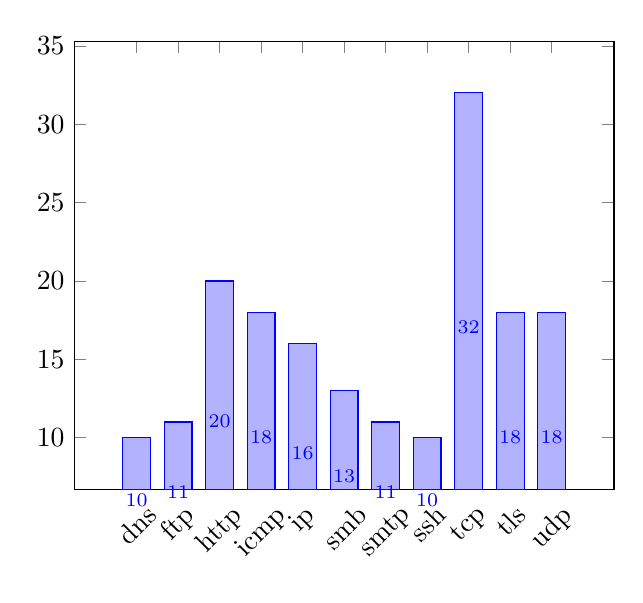
\begin{tikzpicture}
      \begin{axis}[
          ybar stacked,
          enlargelimits=0.15,
          legend style={at={(0.5,-0.15)},
            anchor=north,legend columns=-1},
          %          ylabel={\#rules},
          symbolic x coords={dns, ftp, http, icmp, ip, smb, smtp, ssh,
          tcp, tls, udp},
          xtick=data,
          xticklabel style={rotate=45},          
          nodes near coords,
          every node near coord/.append style={font=\scriptsize},        
          nodes near coords align={vertical},
        ]
        \addplot coordinates {(dns,10) (ftp,11) (http,20) (icmp,18)(ip,16) (smb,13) (smtp,11) (ssh, 10) (tcp, 32) (tls,18) (udp, 18)};
%        \legend{relevant, irrelevant}
      \end{axis}
    \end{tikzpicture}
  }
  \vspace{-2ex}
  \caption{\label{fig:distribution-rules-protocol}Number of relevant
    options per protocol supported by Suricata.}
%\end{wrapfigure}
\end{figure}
  

\subsection{Rules and Packets}
\label{sec:rules-and-packets}

\begin{figure}[h!]
\centering
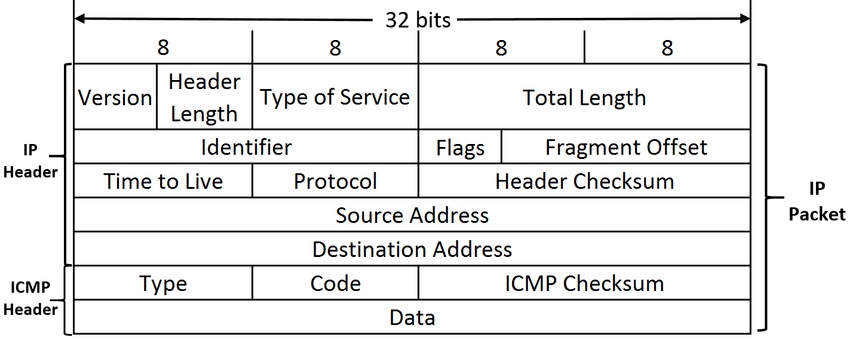
\includegraphics[scale=0.28]{figs/ICMP-packet-structure.png}
\caption{Layout of an ICMP packet.}
\label{fig:icmp-packet-layout}
\end{figure}

Rule options are often associated with specific fields of network
packets. Let's consider the ICMP protocol as an
example. Figure~\ref{fig:icmp-packet-layout} shows the layout of an
ICMP packet. The packet fields ``Flags'' and ``Time to Live'',
declared in the IP header, are mapped to the options \CodeIn{flagbits}
and \CodeIn{ttl}, respectively. Likewise, the fields ``Type'' and
``Code'', declared in the ICMP header, are mapped to the options
\CodeIn{itype} and \CodeIn{icode}. (Table~\ref{table:rules} lists some
example rule options.) The values of the options ``ttl'', ``itype'',
and ``icode'' are the same as the value of the corresponding fields in
the ICMP packet. For the field ``Flags'' the value of the
corresponding option is encoded in the bitvector. For example, if the
``Flags'' field stores the value 1010, the corresponding rule option
will be \CodeIn{flagbits:RM}, as each position of the vector encodes a
different character in the \CodeIn{flagbits} rule option. The value of
several options can be determined through transformation functions, as
those described above. One expection to this is the option
\CodeIn{threshold}, which is typically used in denial-of-service
attacks. That option operates over sequence of messages as opposed to
a single message. Consequently, it is not possible to determined its
values from a single message. More precisely, to trigger an action on
a rule containing that option a \nids\ tool needs to monitor several
messages.

%% \Luc{
%%   Os campos Flags e Time to live no header IP são mapeados para as opções fragbits e ttl, respectivamente. Os campos Type e Code no header ICMP são mapeados para as opções itype e icode. \\
%% Os campos, Time to Live, Type e Code recebem diretamente o valor que está no pacote. Por exemplo, se o campo Type no pacote possuir valor 8, na regra ele vai aparecer como itype:8.\\
%% O campo Flags é intepretado como um vetor de bits, onde cada posição representa uma flag. Na regra, o valor do campo Flags é traduzido em caracteres que representam cada flag presente no pacote. Por exemplo: se o campo Flags possuir o valor 1010, na regra aparecerá fragbits:RM, pois os caracteres R e M indicam a presença do quarto e segundo bits.}


\section{Illustrative Examples}
\label{sec:suri-metas-coverage}

This section briefly presents examples of attacks and illustrates the
rules that \tname{} synthesizes to capture those attacks.


\subsection{Denial-of-Service}

The SYN Flood attack is a denial-of-service attack that exploits a vulnerability in the TCP/IP handshake
to establish a TCP connection~\cite{cloudfare-synflood}. The handshake
works as follows in normal circumstances. First, a client sends a SYN
packet to the server, requesting a connection. Second, the server
responds with a SYN-ACK packet to the client. Third, the client
responds with an ACK message and the connection is established. Aware
of the protocol, an attacker sends multiple SYN packets to different
ports of a server, often using fake IP addresses. Then, after the
server responds with a SYN-ACK packet, the client keeps sending other
SYN packets to avoid the connection to time out. Without proper
protection, the server accepts these malicious requests and eventually
legitimate requests cannot be satisfied due to resource exhaustion.

\begin{figure}[h!]
  \lstinputlisting[language=C,numbers=none,keywords={flags,threshold}]{synflood.suricata}
  \caption{Suricata rule for SYN Flood Attacks.}
  \label{fig:synflood-example}
\end{figure}


Figure~\ref{fig:synflood-example} shows a Suricata rule that captures
this attack. This rule was obtained from the Emerging Threats Open
Ruleset~\cite{emerging-threats-open}. The relevant options in the
rule appear in bold---the option \CodeIn{flags: S,12}, identifies a
SYN packet in a TCP packet and the option \CodeIn{threshold: type
  both, track by\_dst, count 5000, seconds 5} indicates that a high
volume of such packets should be requested in a short period of time.

In the following, we illustrate how \tname{} proceeds for obtaining
the rule for the SYN Flood attack. The challenge in synthesizing rules
is to discover the set of options in a rule that makes the \nids\ to
capture the malicious traffic, but allow the benign traffic to go
through.  The other parts of the rule (\ie{}, the action and the
header) are either inferred or left constant. For example, in this
case, \tname{} sets the action header to \CodeIn{alert} and sets the
header to \CodeIn{<proto> any any -> any any}, indicating that it
infers the target protocol and uses the most general flow description
possible, \ie{}, it instructs the \nids\ to analyze the traffic
flowing from/to any address and port.  We understand that this is
domain-specific information and assume that the system administrator
would know how to customize it.

\tname{} proceeds as follows to synthesize rules for this
attack. First, it analyzes the positive (\ie, malicious) traffic and
extracts options expressed in that traffic. In this case, the
malicious traffic is characterized as a sequence of 20
messages. \tname{} finds the following set of options at this stage:

\begin{figure}[h]
  \vspace{-3ex}
  \lstinputlisting[language=C,numbers=none,frame=none,keywords={flags,threshold,window}]{synflood.suricata.synth}
%  \caption{Suricata rule for SYN Flood Attacks.}
  %  \label{fig:synflood-example-synt}
  \vspace{-3ex}  
\end{figure}

%% \Mar{<~ Lucas/Guilheme, logo acima a gente falou que threshold nao
%%   poderia ser inferido a partir de uma unica mensagem e aqui a gente
%%   fala isto. Vcs. podem explicar o que realmente acontece?}
%% \Luc{O input considerado para ataques de flood eh um conjunto de pacotes e não apenas um pacote unico, nesse caso um conjunto com 20 pacotes. A opção de threshold é incluida na regra quando o input contem mais de um pacote, o parametro count recebe o valor da quantidade de pacotes do conjunto de entrada.}


\Mar{@Lucas/Guilheme, há algo o que remover? talvez ``window:64''?
  Qual a correspondencia de ``flags:S,12'' com ``flags:S''? Por favor,
  respondam isto logo.}  \Gui{O window:64 seria removido sim.}
  \Luc{O segundo campo da opção flags define flags que serão ignoradas. Nesse caso a regra procura por pacotes onde apenas a flag S está 'setada', independentemente do valor das flags 1 e 2. Portanto a regra gerada pode capturar coisas diferentes da regra original. A inferencia do "12" n pode ser feita apenas a partir do pacote de entrada, precisariamos tratar isso.}


\tname{} only reports a rule if the \nids\ (\ie{}, Suricata)
instantiated with that rule is able to capture the traffic passed on
input. Consequently, by construction, a rule that uses this set of
options captures the malicious traffic. Unfortunately, this rule is
potentially overspecified. Informally, the rule includes ``too many''
characteristics of the malicious traffic used to define it and could
potentially result in false negatives.

Second, \tname{} uses negative (\ie{}, benign) traffic to address the
overfitting issue. \tname{} searches for alternative rules that
preserves the invariant that a rule should only capture the positive
traffic. It uses the rule obtained in the previous step to bootstrap
the search.

Finally, \tname{} ranks the inferred rules according to heuristics
extracted from a database of existing \tname{} rules. One example
heuristic is \Fix{...informa um exemplo concreto que
  vc. usaram...}. Instead of traffic, this step looks for the
structure of existing rules. The list below shows the rule options for
the top-5 rules \tname{} produces for this attack.

\Mar{listem 5 primeira regras neste caso}


\subsection{Active Reconnaissance}

Active reconnaissance is a method used by malicious individuals to
collection information about a computing system to determine potential
vulnerabilities. Active reconnaissance is a preliminary step towards
an actual attack. The most popular technique is to ``scan'' open ports
in a host. A Ping Scan is a very common type of port scan based and it
is based on the ICMP protocol. \Mar{@Lucas, acima falamos de
  porta. Abaixo nao falamos de porta, apenas de maquina. Vc. pode ser
  mais especifico? ->}
  \Luc{De fato estamos falando de duas coisas diferentes, mas ambas são exemplos de 'active reconnaissance'. Primeiramente citamos o port scanning, q tem o objetivo de encontrar portas abertas em uma maquina especifica. Depois falamos do ping scan, q tem o objetivo de encontrar ip's ativos numa rede.} To scan a network, an attacker sends a several
ICMP Echo requests addressed to a range of IP addresses in the network
and checks which ones respond to the requests. This allow the attacker
to know which machines are active in the network, then it can choose
one of them to attack.

\begin{figure}[h!]
  \lstinputlisting[language=C,numbers=none,keywords={dsize,itype}]{pingscan.suricata}
  \caption{Suricata rule for Ping Scan.}
  \label{fig:synflood-example}
\end{figure}

Figure 4 shows a Suricata rule that captures a ping scan implemented
with NMAP~\cite{netmap}, a network discovery and security auditing
open-source tool. The relevant options are in bold---the option
\CodeIn{dsize: 0} indicates that the packet has no bytes in the
payload and the option \CodeIn{itype: 8} indicates that the packet to
be captured are ICMP Echo requests.

Again, to synthesize rules for a Ping Scan, \tname{} analyzes the
positive traffic and extracts the following rule options:


\begin{figure}[h]
  \vspace{-2ex}
  \lstinputlisting[language=C,numbers=none,frame=none,keywords={dsize,icode,itype}]{pingscan.suricata.synth}
  \vspace{-3ex}  
\end{figure}


Again, note that rule \CodeIn{icode} was not present in the original
rule.  \tname{} produces the following five rules at the top of the
ranking after minimization and ranking.

\Fix{...show rules...}

\subsection{\Fix{Name of attack ***with content***}}
\label{sec:content-example}

\Fix{...please elaborate. We need on example that shows that the
  search can be non-trivial. In the examples above, we had to discard
  only one rule option!}


%% \begin{table}[h]
%%   \caption{\label{table:rules}Rule evolution}  
%%   \centering
%%   \begin{tabular}{lllll}
%%     \toprule
%%     \multicolumn{1}{c}{Iteration} & \multicolumn{1}{c}{Rule} \\
%%     \midrule     
%%     0 & (ack:0; seq:0; window:0; flags:F;)\\
%%     5 & (window:0; flags:F;)\\
%%     68 & (window:64; flags:F;)\\
%%     73 & (window:64; flags:S,12;)\\
%%     94 & (window:64; flags:S,12; threshold: type both, track by\_dst, count 20, seconds 1;)\\
%%     \bottomrule
%%   \end{tabular}
%% \end{table}

\section{Technique}

\tname{} is a technique to synthesize signature-based rules for
\nids~(\eg{}, Snort~\cite{snort} and Suricata~\cite{suricata}). The
goal of \tname\ is to create rules that captures \emph{only} the
malicious messages. 

\begin{figure*}[t]
\centering
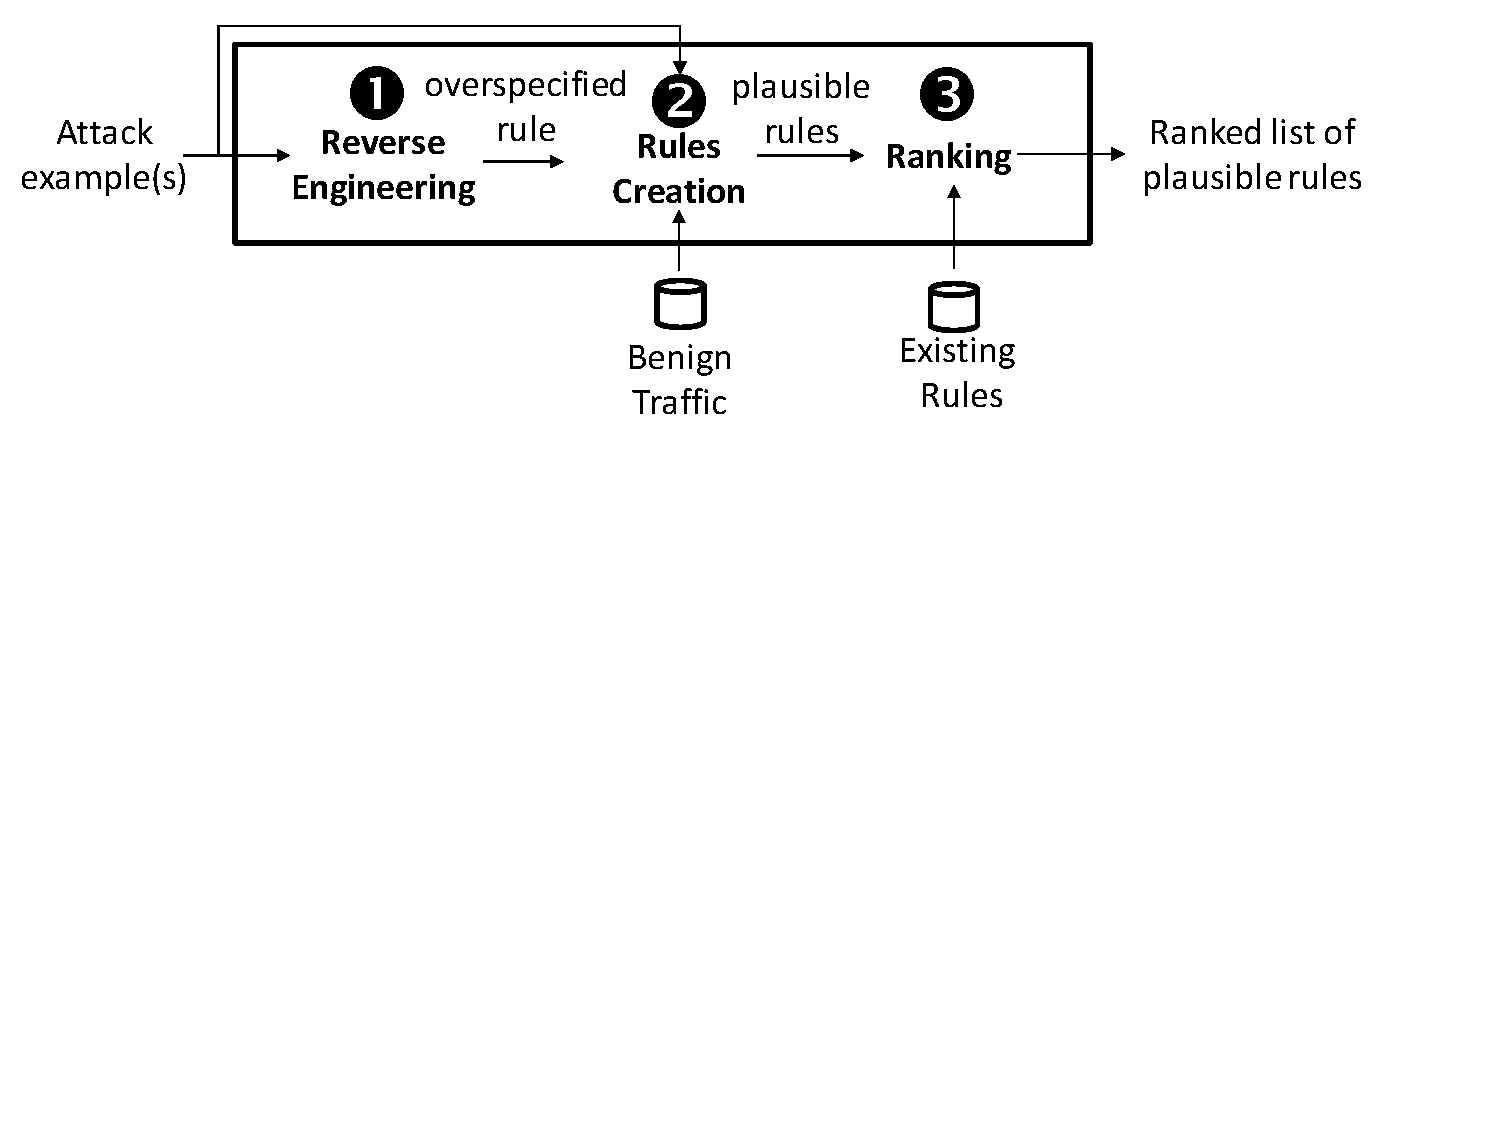
\includegraphics[trim=0 350 100 0,clip,width=0.65\textwidth]{figs/nids-workflow}
\caption{\tname\ workflow.}
\label{fig:overview}
\end{figure*}

\vspace{1ex}
\noindent\textbf{Overview.}~To create rules, \tname\ leverages (1)
benign and malicious network traffic and (2) rules from public
rulesets. Figure~\ref{fig:overview} shows the workflow of \tname{} as
a pipeline of three components, which appear numbered in the figure.
The inputs of the technique appear at the bottom of the figure whereas
the output appear at the right. \tname\ takes on input malicious and
benign traffic and a set of rules from public rulesets and produces on
output a list of plausible rules to isolate the malicious traffic.

\tname\ works as follows. First, it produces a potentially
overspecified rule that captures the malicious traffic, provided on
input in the form of pcap files~\cite{pcap}. In this step,
\tname\ detects rule options in correspondence with the input messages
(see Section~\ref{sec:rules-and-packets}). It is worth noting that the
rule produced in this step can include more options than the golden
rule (see Section~\ref{sec:suri-metas-coverage}). Consequently, the
use of that rule could lead, in principle, to false negatives as not
all manifestations of the same attack are identical, \ie{}, the
content of messages for two instantiations of a given attack may
differ. Second, \tname{} generates plausible rules similar to the one
produced in the previous step. It is worth noting that any subset of
the original set of options captures the malicious traffic. As the
generation procedure discards options from the initial rule, it
satisfies the invariant of capturing malicious traffic by
construction. However, the goal of \tname\ is to produce rules that
capture \emph{only} malicious traffic. To achieve that goal, \tname{}
uses benign traffic from public databases to check that the
\nids\ instantiated with a given rule does not capture benign
traffic. The minimization step uses a population-based gradient
descent-like search to find all plausible rules, which are derived
from the rule obtained in the previous step. Third,
\Fix{...elaborate...}



%% The goal of the first
%% component is to produce a rule that captures the negative traffic.
%% First, it initializes the rule with random values. Only options
%% associated with the used protocol are included in the rule
%% representation. Then, \tname\ optimizes the rule options until
%% \suri\ is able to capture the attack associated with the negative
%% traffic.  \tname\ unsuccessfully terminates at this point if it cannot
%% capture the attack. The second component takes as input the rule
%% produced by the first component and tries to minimize that rule. Note
%% that any subset of options would capture the negative traffic---as all
%% options in the rule need to be satisfied for the negative traffic to
%% be captured---but it can also capture positive traffic. This component
%% systematically discards options from the rule encoding until no
%% positive traffic is captured.



\subsection{Step 1: Reverse Engineering}




\pgfplotsset{width=6cm,compat=1.8}
\pgfplotsset{every tick label/.append style={font=\tiny}}

%\begin{wrapfigure}[15]{r}{0.56\textwidth}
\begin{figure}[t!]
  \centering
%  \vspace{-4ex}
  \scalebox{1.2}{  
    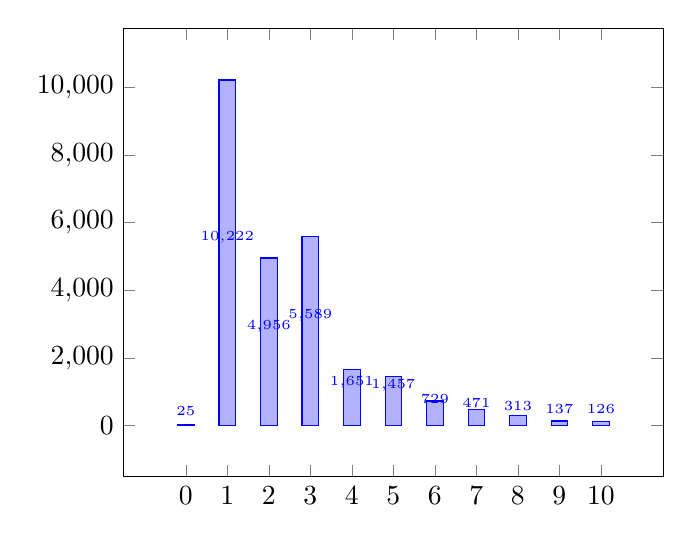
\begin{tikzpicture}
      \begin{axis}[
          bar width=6pt,
          scaled ticks=false,
          tick label style={/pgf/number format/fixed},
          ybar stacked,
          enlargelimits=0.15,
          legend style={at={(0.5,-0.15)},
            anchor=north,legend columns=-1},
          symbolic x coords={0, 1, 2, 3, 4, 5, 6, 7, 8, 9, 10},
          xtick=data,
          nodes near coords,
          every node near coord/.append style={font=\tiny},
          nodes near coords align={vertical},
        ]
        \addplot coordinates {(0,25) (1,10222) (2,4956) (3,5589)
          (4,1651) (5,1457) (6, 729) (7, 471) (8, 313) (9, 137) (10, 126)};
      \end{axis}
    \end{tikzpicture}
  }
  \caption{\label{fig:distribution-contents}Histogram of number of
    \CodeIn{content} options per rule (up to 10).}
%\end{wrapfigure}
\end{figure}  



The goal of the first step is to extract options from the positive
traffic. For that, \tname{} parses the protocol message, looking for
fields in the message associated with options (see
Section~\ref{sec:rules-and-packets}).
Unfortunately, inferring options at the field granularity
level is insufficient to capture \CodeIn{content} options (see
Section~\ref{sec:example-suricata-rules}), which refer to parts of the
payload of the message and cannot be directly extracted directly from
the fields. Handling this case is critically important as most rules
contain \CodeIn{content}
options. Figure~\ref{fig:distribution-contents} shows the histogram of
number of these options per rule (up to 10) obtained from a public
ruleset~\cite{emerging-threats-open} containing 27.8K Suricata
rules. Rules without \CodeIn{content} options is an exception and half
of the rules contain at least two \CodeIn{content} options.  To find
the values associated with these options, \tname{} splits the payload
of the malicious message in tokens using natural language delimiters,
such as $\backslash$t, $\backslash$n, $\backslash$r, and spaces. The
rationale for this decision is that we observed, by inspecting
existing rules, that \CodeIn{content} options typically refer to
sequence of characters in the payload of messages separated by these
delimiters. This tokenization step can generate dozens of options. For
the example from Section~\ref{sec:content-example}, \tname{} produces
a total of \Fix{xx} content options.


\subsection{Step 2: Rule Minimization}
\label{sec:minimization}

The rule reported in the first step satisfies the criterion to only
capture positive traffic. Unfortunately, the rule produced in the
first step is overconstrained---it is unable to capture different
manifestations of the same attack as the rule matches all options that
\tname\ found for the input message.

%%  Some options added to the rule
%% during the first step are irrelevant for determining the attack and
%% should be removed to obtain more general rules. 

\tname{} leverages public datasets\cite{tcpreplay} of negative traffic
to guide the search for more general rules, hence addressing the
overffiting issue. The goal of this step is to create rules that
captures traffic similar to the input malicious traffic. To achieve
that goal, \tname{} \emph{minimizes} the rules produced in the
previous step, preserving the invariant of \emph{only} capturing the
positive malicious traffic. A rule is minimal if discarding any option
results in capturing negative (\ie{}, benign) traffic.  The
minimization procedure we propose in this step builds on the
observation that all options from the rule produced in the previous
step are satisifed by the positive traffic. Consequently, any subset
of these options also captures the positive traffic. The procedure
iteratively discards options from the candidate rule until it detects
that the rule is minimal, \ie{}, it finds that no other option can be
removed. The procedure uses negative traffic to guide the search.



\algdef{SE}[DOWHILE]{Do}{doWhile}{\algorithmicdo}[1]{\algorithmicwhile\ #1}%
\algnewcommand\algorithmicforeach{\textbf{for each}}
\algdef{S}[FOR]{ForEach}[1]{\algorithmicforeach\ #1\ \algorithmicdo}
\algnewcommand\And{\textbf{and} }
\begin{algorithm}[t!]
  \noindent\hspace{-31ex}
  \textbf{INPUT:} overconstrained rule $or$ \\
  \noindent\hspace{-30ex} 
  \textbf{OUTPUT:} Set of minimal rules $\mathcal R$\\
%\vspace{-3ex}
\captionof{algorithm}{Minimization algorithm}\label{algo1}
\begin{algorithmic}[1]
  \State $\mathcal R \gets \{\mathit{or}\}$\Comment{initial population
    of candidate solutions contains only the input rule.}\label{line-init}
  \Do\label{start-do-while}
      \State $\mathcal R' \gets \emptyset$ \Comment{starting new
        iteration. new generation should be empty.}\label{init-rprime}
      \ForEach {$ro \in \mathcal R $}\Comment{analyze each candidate individual/rule separately.}\label{start-foreach}
           \For {$i \gets 1$ to $N$}\Comment{mutate each rule $N$ times.}\label{start-for}
               \State $r \gets copy(ro)$      
               \State $j\gets \mathit{rand}(0,\mathit{len}(r))$
               \State $r[j]\gets 0$\Comment{discard option $j$ of rule
                 $r$, a copy of the original rule $\mathit{ro}$}
               \If{$\mathit{isnew(r)} \And \mathit{isfit}(r)$} 
                   \State $\mathcal R' \cup\gets \{r\}$\Comment{$r$
                     can lead to a plausible candidate solution.}\label{line-progress}
               \EndIf
           \EndFor\label{end-for}
       \EndFor\label{end-foreach}
       \State $\mathcal R \gets R'$\Comment{update new generation}
  \doWhile{$\mathcal R'\not= \{\}$}\Comment{repeat until reaching a fixpoint}\label{end-do-while}
\end{algorithmic}
\end{algorithm}

Algorithm~\ref{algo1} shows the pseudocode of the \tname{}
minimization algorithm. The algorithm takes as input the
overconstrained rule produced by the reverse engineering step and
produces a set $\mathcal R$ of rules that are minimal and only
captures the positive traffic. Line~\ref{line-init} initializes the
set $\mathcal{R}$ of candidate solutions with the input rule $or$. We
encode a rule as a bitvector where each index in the vector represents
one option; the value assigned at a given position indicates whether
or not the option is present in the rule. Each iteration of the outer
loop (lines~\ref{start-do-while}-\ref{end-do-while}) represents one
generation of the population of individuals produced by the
search. The algorithm terminates when no rule in the current
generation of individuals could be further reduced without violating
the property that a candidate solution should only capture positive
traffic. This means that execution has not reached
line~\ref{line-progress} as to augment the set $\mathcal{R'}$ and that
set will be empty at the end of one iteration of the outer
loop. Line~\ref{init-rprime} initializes the new generation of
candidate rules. The loop from
lines~\ref{start-foreach}--\ref{end-foreach} iterates through each
candidate rule in $\mathcal R$. Note that these rules have been found
in the previous generation. The algorithm mutates each of these rules
for $N$ times, discarding one option of the rule each time. The call
to $\mathit{isNew}$ checks if $r$ has not been previously generated
through another path whereas the call to $\mathit{isfit}$ checks if
the rule only captures positive traffic. Function $\mathit{copy}$
creates a copy of the bitvector of a rule, function $\mathit{len}$
returns the length of the vector, and function $\mathit{rand}$
randomly chooses one index of the vector.

\begin{theorem}
  The minimization algorithm computes rules that capture only
  the positive traffic.
\end{theorem}
\begin{proof}
  Every rule created during the search captures the positive traffic
  as every rule contains a proper subset of the option from the
  original rule and all those options are satisfied by the positive
  traffic. By definition of function $\mathit{isfit}$, these rules
  also capture \emph{only} the positive traffic. If some negative
  traffic was captured, a rule would not be added to $\mathcal
  R'$.\qed
\end{proof}

\begin{proposition}
  The minimization algorithm may not produce minimal rules.
\end{proposition}

The output of the minimization algorithm may contain rules that are
not minimal given the non-determinism of the algorithm. It is possible
that options that could be discarded are not selected in the loop from
lines~\ref{start-for}--\ref{end-for}. However, we found empirically
that a small value of $N$ suffices to produce minimal rules.

%% Public databases of negative traffic with
%% \Fix{thousands} of messages exist  and can be used to
%% increase the accuracy of the minimization.
%\subsection{Limitations}
%\Fix{...}

\vspace{2ex}
\noindent\textbf{Limitation.} It is worth noting that although
\tname{} is accurate for generating rules that discrimate positive and
negative traffic, the quality of these rules is limited by the quality
of the training data it uses. For the positive traffic, \tname{} only
requires one sample, but can benefit of several samples. For the
negative traffic, \tname{} can use public datasets available online.

\vspace{2ex}
\noindent\textbf{Implementation details.} We implemented function
\emph{isFit} by 1)~updating Suricata to only use the informed rule,
2)~replaying the negative traffic (see
Section~\ref{sec:dataset-benign}), and 3)~reading the Suricata logs to
check if any benign message was captured by the rule. It is worth
noting that the benign traffic is stored in ``pcap'' files~\cite{pcap}
and Suricata can process those files very efficiently compared to
analyzing network messages directly.

\section{Evaluation}

This section evaluates the precision and efficiency of \tname{}.

\subsection{Objects of Analysis}

Table~\ref{table:attacks} shows the attacks we analyzed and the
options of the rule from the Emerging Threats Open
Ruleset~\cite{emerging-threats-open} that captures the attack. Column
``Name'' shows the name of the attack, column ``Protocol'' shows the
protocol name, and column ``Ground Truth'' shows the options of the
rule that captures the attack.

\begin{table*}[h]
  \caption{\label{table:attacks}List of attacks.\Mar{Guilherme, por
      favor, adicione mais ataques aqui...}}
  \centering
  \begin{tabular}{lll}
    \toprule
    \multicolumn{1}{c}{Name} &
    \multicolumn{1}{c}{Protocol} &
    \multicolumn{1}{c}{Groud Truth} \\
    \midrule     
    Ping Scan \MyComment{& single} & ICMP \MyComment{& Discovers
      active hosts in a network} & \scriptsize{dsize:0; itype:8;} \\
    Black Nurse \MyComment{& multiple} & ICMP \MyComment{& Denial of Service} & \scriptsize{itype:3; icode:3; detection\_filter:track by\_dst, count 250, seconds 1;}\\
    Ping Flood  \MyComment{& multiple} & ICMP \MyComment{& Denial of Service} & \scriptsize{itype:8; icode:0; detection\_filter:track by\_src, count 30, seconds 1;}\\  
    Port Scan \MyComment{& single} & TCP \MyComment{& Discovers open ports in a host} & \scriptsize{flags: A; ack: 0;dsize: 0;} \\
    SYN Flood \MyComment{& multiple} & TCP \MyComment{& Denial of Service} & \scriptsize{flags: S,12; threshold: type both, track by\_dst, count 5000, seconds 5;}\\
    UDP Flood \MyComment{& multiple} & UDP \MyComment{& Denial of Service} & \scriptsize{fragbits:M; threshold: type both, track by\_dst, count 5000, seconds 5;} \\
    \bottomrule
  \end{tabular}
\end{table*}

\subsection{Dataset of Benign Traffic}
\label{sec:dataset-benign}

Note from Figure~\ref{fig:overview} that the positive traffic is an
input to the technique. The negative non-malicious traffic, however,
is not. \tname{} uses public databases storing different kinds of
positive traffic for all protocols covered by Suricata. We used two
datasets of positive traffic. The Bigflows.pcap dataset is part of the
TcpReplay~\cite{tcpreplay} open source project. This dataset includes
real network traffic on a busy private network access point to the
Internet. According to the TcpReplay web site ``This capture is much
larger and has a smaller average packet size than the previous capture
(smallFlows.pcap). It also has many more flows and different
applications.''. In addition to the Bigflows.pcap dataset, we also
used datasets of normal traffic made available by Stratosphere
Lab~\cite{stratosphere-normal}.

\subsection{Methodology}

\tname{} expects (a) message(s) reproducing an attack on input. As
previously discussed, those messages could be directly provided by an
anomaly-based \nids\ tool. To evaluate \tname{}, however, we created
those messages ourselves. For all attacks listed on
Table~\ref{table:attacks}, we found reproduction scripts available on
the web. With the script to reproduce the attack, we proceeded as
follows: 1)~we instantiated the script on a given target machine,
2)~we executed the script, 3)~we monitored the traffic with the
wireshark network monitor~\cite{wireshark-net-monitor}, and 4) we
simulated the delivery of the corresponding network messages by
directly executing Suricata on the ``pcap'' files that wireshark
produced in the previous step. It is worth noting that Suricata is
invoked multiple times in the process of minimizing the rule (see
Section~\ref{sec:minimization}) and that processing pcap files is much
more efficient compared to sending and processing network messages. To
illustrate, the SYN Flood attack was reproduced with the hping3
tool~\cite{hping3} using the following command \CodeIn{hping3 -d 80 -w
  64 -S -p 80 --flood --rand-source <IP>}.

%% \Gui{We are using the bigflows.pcap provided by tcpreplay on http://tcpreplay.appneta.com/wiki/captures.html "This is a capture of real network traffic on a busy private network’s access point to the Internet"
%%  }

%% \Luc{entrada: utilizamos a ferramenta hping3 para executar o ataque em um alvo arbitrario dentro da rede (n ha necessidade de haver um alvo real para executar o hping3) e capturamos o trafego gerado com o wireshark. o comando utilizado foi:\\*
%% \texttt{\# hping3 -d 80 -w 64 -S -p 80 --flood --rand-source 192.138.1.115} \\*
%% que envia pacotes de 80 bytes (-d 80), com a flag SYN habilitada (-S), tamanho de janela de 64 bytes (-w 64), direcionados a porta 80 (-p 80). A flag --flood indica q o hping3 vai enviar os pacotes o mais rápido possível. a flag --rand-source indica que cada pacote vai ter um ip de origem aleatorio. 192.138.1.115 é o alvo.\\*
%% O trafego armazenado contem 40 mil pacotes SYN, enviados no intervalo de 1 segundo,  pegamos uma amostra de 20 desses pacotes para representar o flood e servir como entrada.\\*
%% O wireshark armazena os pacotes no formato pcap, utilizamos a ferramenta tcpreplay para reproduzir o trafego com o comando:\\*
%% \texttt{\# tcpreplay --pps 200 --intf1=wlp2s0 Datasets/syn-flood-sample.pcap}\\*
%% Nesse caso, estamos enviando os pacotes armazenados em \texttt{Datasets/syn-flood-sample.pcap} a uma taxa de 200 pacotes por segundo (\texttt{-pps 200}) utilizando a interface wlp2s0 (\texttt{--intf1 wlp2s0})\\* 
%% Há diferenças entre os pacotes na opção ack.\\* 
%% Por que 20? Apenas para gerar a regra mais rapidamente, poderia ser qualquer valor maior ou menor. No final, o parâmetro \texttt{count} da opção \texttt{threshold} vai ser alterado pelo adm da rede.\\*
%% Intervalo de reprodução: 0.005 segundo

%% }

%% \Fix{any other detail we should consider?}

\subsection{Precision}

\Fix{}

\subsection{Efficiency}

\subsection{Threats to Validity}

External Validity. \Fix{elaborate ...how popular are Suricata/Metasploit?}

\section{Related Work}

\Fix{...}

\section{Conclusions}

\Fix{...}

%% \section*{Acknowledgments}
%% This work is partially supported by RNP grant number 002951.


\bibliographystyle{ACM-Reference-Format}
\bibliography{references}

\end{document}
\endinput
%%
%% End of file `sample-sigconf.tex'.
